%----------------------------------------------------------------------------------------
%	PACKAGES AND OTHER DOCUMENT CONFIGURATIONS
%----------------------------------------------------------------------------------------
\documentclass[11pt]{report}

\usepackage{lastpage} % Required to determine the last page for the footer
\usepackage{extramarks} % Required for headers and footers
\usepackage{graphicx} % Required to insert images
\usepackage{lipsum} % Used for inserting dummy 'Lorem ipsum' text into the template
\usepackage{hyperref}
\usepackage{float}
\usepackage[bottom]{footmisc}
\usepackage{subcaption}

\linespread{1.1} % Line spacing
\usepackage[total={6in, 8in}]{geometry}

\setlength\parindent{0pt} % Removes all indentation from paragraphs

\begin{document}
\title{Novel Gaming Experiences with Advanced Illumination 
through Augmented Reality: Interim Report}
\author{Terence Tse \\
		Supervisor: Benjamin Glocker\\
		Second Marker: Abhijeet Ghosh}
\maketitle
\newpage

\newpage

\section*{Abstract}

\newpage

\section*{Introduction}
\begin{center}
\textit{I want to create the world.}
\end{center}

Augmented Reality(AR) has come into the limelight once again with the recent release
of the Google Glass. AR has been around for a while now, most of the time being
thought of the future of technology but with applications ending up with 
limited use, less than satisfying performance and being gimmicky, it has been
hanging around in the background for a while.
\\ \\
AR in a nutshell is reality, augmented! A view of the real world is presented
to the user but it has been enriched in some sort of way. If you are unaware
of what looking through a Google Glass is like, one pretty well known example 
is the film Terminator. When seeing from Terminator's viewpoint, we are 
presented with a red screen, this is what a normal person would see but in red.
However, on the screen, it has a crosshair, which lock onto a person, their
statistics in the right hand corner, when it's your target, the words flash
in view. This is what augmented reality is.
\\ \\
Of course, we're not all cyborg assassins, hence why things like the Google 
Glass have been created. Our eyes already give us a lot of information about 
the world, but having even more information presented to us than what we
naturally have is Augmented Reality. Already, anyone with a semi-decent mobile
phone can play around and take benefits from Augmented Reality, it does not take
large amounts of processing power to produce an AR image. The key is that AR is
real time, our view gets updated as we see it. 
\\ \\
Augmented Reality is not just limited to some head mounted device. In addition
to our phones, we can use tablets or just plain computers in which to play
with AR. All we need is a camera which can capture the world and then allow 
us to view it either with additional information or even diminished information!
One use case is in the British Maritime museum, where visitors can aim cameras
at special AR exhibits and have the item explained to them visually. The range 
applications of AR are overwhelming, imagine a Dinosaur coming to life in a
History museum and you can see it navigating the halls. Imagine having an
AR mirror that superimposes clothes onto your body that fit, without having
to go and search and try on the clothes themselves. Imagine being on a 
construction project and you are able to view the outcome on your tablet, even
if the old structure has not been cleared away for the new project to begin!
Augmented Reality can do all of that already and the scope of new
applications is, no pun intended, as far as the eye can see!    
\\ \\
As previously stated, AR has many applications in terms of games and 
entertainment. These come in all different styles, from simple use of a camera,
to using fixed feature points as markers, or using patterns as feature points
to identify placement of objects in the scene. Right now, these feature points
are either very simple or immutable. They are something that the computer
can directly identify which is obviously good for performance reasons. However,
what about the ability to create your own feature points on the fly? If we
able to immediately draw feature points and by extraction of these points, 
augment reality based off of these points, it would greatly improve the 
experience of Augmented Reality, removing the need to create the marker 
on a computer and just, for example, grabbing a piece of paper, drawing it
yourself and have it work straight away! I shall refer to this as a feature
drawing throughout the rest of the report. 
\\ \\
However, AR may also be used for more commercial and other practical uses. 
When people think of AR, it usually defaults to thinking about games and 
indeed there is a lot of future in that industry with AR, there are also
Educational uses, Project and Landscape Planning, Commerce and Animation, 
the list goes on. The problem right now is that simple AR applications which
augment a scene with, say a dinosaur or some other object, those generated
images are still quite obviously generated by a computer, especially when 
they try to get more complex. In a bright room, you may place furniture inside
which looks semi-realistic, it has a computed shadow and gradient change. 
However, an ideal situation is when we augment reality and it doesn't even
feel as if anything is different. In other applications, the objects may not
even have an advanced lighting model, solid colours with no depth or 
obscurance may be modelled, thus not even a shadow is created making it 
extremely obvious (whether this is desired or not) to us which objects in
the scene have been artificially generated. It is harder to appreciate this
as an extension of reality when it is so obvious that this object does not
belong in the scene.
\\ \\
This project is focused around these points. First, I'd like to make additions
to the AR realm; I will focus around using Augmented Reality to 
provide not only a novel gaming experience, but also one that can be 
transferred over to more practical use cases while appearing realistic in
addition to have users generate a set of feature points manually in the real scene.
One way that we can drastically improve the realism of a computer generated
image is to improve the illumination model to such a degree that the object
looks like it belongs in the view. 
\\ \\
\subsection*{Project Goals}
The bigger picture and where this project hopes it can contribute and make 
headway into is permitting a dynamic and responsive AR application that allows
creators to quickly draw up environments which can then be visualised. 
Environments can also be changed in real time and will be reflected in the AR
without need for additional user interaction. The completion of this
task will have numerous transferable benefits that were mentioned in the 
SECTION ABOVE. %FILL THIS IN

However, the amount of work that this goal encompasses coul be infintissimal
depending on what kind of features would be deemed necessary, good or just an
extension. There are also numerous parts of a project like this could be 
analysed in much further detail. As a result, the objectives for this project
are:

\begin{itemize}
	\item Create a functioning Augmented Reality program which takes a
		  video stream and overlays a 3D landscape on a contour map created by
		  the user. The contour map may also have other feature points which 
		  indicate other 3D structures to be rendered.
	\item Using a method of video and scene tracking/recognition, allow users
		  to make changes to their contour map and have the landscape update 
		  in real time. This essentially allows dynamically changing 
		  Augmented Reality landscapes.
	\item Perform an analysis on the performance and responsiveness 
		  of the final product of this project. This will be done
		  through user testing.
		 
\end{itemize}

\newpage
\section*{Background}

\subsection*{Augmented Reality}
\begin{center}
What is Augmented Reality(AR) and why should we be interested in it? \\
\end{center}
In recent years, it becomes harder and harder to concisely describe what
constitutes as Augmented Reality. The reason for this being that as technology
improves more and more things are being achieve that allow users to extend
their perceived reality with extra data.\\ 

Simply put, Augmented Reality is when the environment around you can be 
extneded by combining both real and virtual data components. Azuma's 
paper\cite{Azuma97}, \textit{A Survey of Augmented Reality},
describes AR as having the following three characteristics:
\begin{enumerate}
	\item Combines Real and Virtual (data) 
	\item Interactive in real time
	\item Registered in 3D
\end{enumerate}

While these are the basic things that constitute AR, there are three ways, 
outlined in Mackay's paper\cite{Mackay}, \textit{Augmented reality: linking 
real and virtual worlds: a new paradigm for interacting with computers},
in which you can augment reality.\\
These are:
\begin{enumerate}
	\item Augmenting the User
	\item Augmenting Physical devices/objects
	\item Augment the Environment
\end{enumerate}

\underline{Augment the User} \\
Augmenting the user is having the user carrying, wearing or using a device
that provide the user with extra information. When we talk about augmenting
the user, the devices we talk about are usually
heads-up displays (HUDS) which the user will have a screen in front of their
eyes in some shape or form. One example of this is Google Glass, allows
users to project information about what they see or their GPS location onto
parts of the glass. If the user was looking at the Eiffel Tower through their 
glass, with GPS coordinates and a scan of the shape of the Eiffel Tower, 
Google Glass would be able to tell that what the user was looking at. From there,
it can project information about the landmark to the user which would not have
been accessible so easily otherwise! \\

This is one such trivial application of
user worn AR, it is very useful for lesser known things, for example, instead of 
looking at a famous landmark, the user could be an engineer, looking at a 
complex piece of machinery and a HUD allowing them to get information on each
component. This is also being trialled in Medicine, where doctors can use
Augmented Reality to help teach surgical procedures or even help them in
analysis of medical images such as X-Rays.\\

\underline{Augment Devices} \\
When an object or device has a small computer placed into it, it can be 
considered as an augmented device. One example of this is again in 
surgery and medical environments. Having tools such as scalpels or other 
medical equipment fitted with computers to plot out how much of the skin has
to be cut, for example, allows the user to receive much more information
than they would be able to than without. Mackay also talks about these briefly 
in her paper.\\

\underline{Augment the Environment} \\
This form or AR doesn't add any additional hardware to devices nor the user.
It focuses on having external devices, such as projectors or cameras take 
input from the user and use that to transofrm the environment that they are in
or are manipulating. This class of AR is much wider than the two 
aformentionned as there are less things imposed on an object/person which 
allow a larger spectrum of devices to be used. \\

An example of Augmenting the environment is an AR keyboard, a projector displays
a keyboard in front of where it is placed, the user can then "press" keys and
the kyboard will be able to detect which key has been selected and translate it 
into computer input. \\

A more common device is your smart phone! Tablet or even computer screens can
be included in this form of AR. There are plenty of mobile applications that
allow users to experience AR in their own unique way. An example used in the
British Maritime Museum is the ability to take a tablet with predownloaded apps
that allow users to engage in an AR game. Through the game, which is primarily
aimed at children, allows them to learn about the exhibits in a more fun and
interactive way. There are also similar applications in retail, for example
in retail! Augmented reality mirrors are being used to avoid the time in the
changing room and allow customers to "try" on pieces of clothing through
AR by overlaying the garment over their captured video. \\

Another fun implementation of AR is the Augmented Sandbox. A projector and
a camera are used to transform a sandbox into a remoldable landscape. The camera
uses depth sensing and the input from here is transformed into lanscape height
and the projector correspondingly projects land or water onto these areas. The
magic happens when the sand is manipulated and the whole system re-renders the
landscape in real time to provide an interactive augmented environment! Sarah
Reed from the University of California lead the authoring of the persentation
about this piece of tehnology\cite{Reed14}.\\




\subsection*{Computer Vision and Image Processing}
A key part of this project is the Computer Vision aspect. The field of
Computer Vision involves the understanding of data from images and pictures.
Understanding is a broad term that encompasses many ways of manipulating or
processing images in order to extract features or points of interest that
can be then used by the computer.

\subsubsection*{Edge Detection}
% Detecting lines and edges of paper, for registration
A key part of Computer Vision is line and edge detection. Edge detection is
the very beginning of how we can start to identify different objects 
within an image. In addition, by stripping an image down to its comprising
edges, we greatly decrease the amount of information in the image whilst
preserving the important parts which we want to operate on.
As a result, how edges are detected have a large contribution
to what we can do with certain images. There have been 
numerous methods of detecting edges put forward, some Gradient-based and
Laplacian based edge detection methods are outlined in 
\textit{A Comparison of various Edge Detection Techniques used in Image Processing}
\cite{Shriv12}. The edge detector used by the Computer Vision Library, 
openCV, is the Canny Edge detector, put forward by John Canny in his paper
\textit{A Computational Appraoch to Edge Detection}\cite{Canny86}. The paper
dicusses a methematical approach to edge and ridge detection which is then
analysed on in Ding and Goshtasby's paper, 
\textit{On the Canny Edge Detector}\cite{Ding00}.





\subsubsection*{Canny Edge Detector}
% Detecting Contours for landscaping



\subsubsection*{Open and Closed contours}
We understand a closed contour to be a loop. By this we mean that if we had
to draw a closed contour, we begin at a point on a piece of paper and end at that
point, either by not removing our pen from the page or, if done so, will resume
at the same point to finish up the contour. The existence of white space between
points on a contour mean that the contour is open, thus not closed. Examples
of open and closed contours can be seen in Figure \ref{fig:closedcontours} and 
Figure \ref{fig:opencontours}.
\\

\begin{figure}[!ht]
	\centering
	\begin{subfigure}[t]{.3\textwidth}
		\centering
		
\includegraphics[scale=0.3]{pics/closedloop1.png}
		\caption{Contour is fully closed, no gaps}
	\end{subfigure}
	\hfill
	\begin{subfigure}[t]{.3\textwidth}
		\centering
		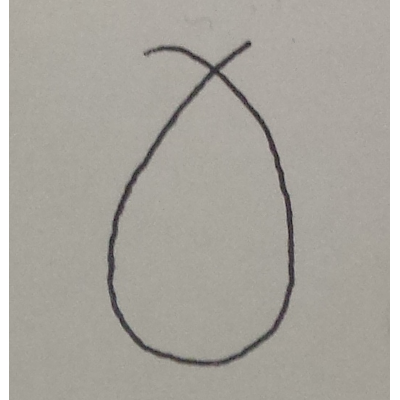
\includegraphics[scale=0.3]{pics/closedloop2.png}
		\caption{Contour is closed, but with artefacts on the ends}
	\end{subfigure}
	\hfill
	\begin{subfigure}[t]{.3\textwidth}
		\centering
		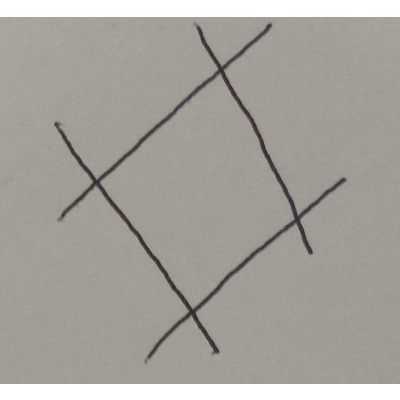
\includegraphics[scale=0.3]{pics/closedloop3.png}
		\caption{This is also a closed contour}
	\end{subfigure}
	\caption{Examples of \textbf{closed} contours}
	\label{fig:closedcontours}
\end{figure}

\begin{figure}[!ht]
	\centering
	\begin{subfigure}[t]{.3\textwidth}
		\centering
		
\includegraphics[scale=0.3]{pics/openloop1.png}
		\caption{A line/edge counts as an open contour}
	\end{subfigure}
	\hfill
	\begin{subfigure}[t]{.3\textwidth}
		\centering
		
\includegraphics[scale=0.3]{pics/openloop2.png}
		\caption{Contour open as beginning doesn't connect to end}
	\end{subfigure}
	\hfill
	\begin{subfigure}[t]{.3\textwidth}
		\centering
		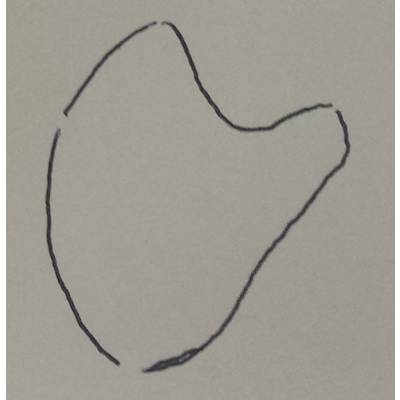
\includegraphics[scale=0.3]{pics/openloop3.png}
		\caption{This contour is open with several gaps}
	\end{subfigure}
	\caption{Examples of \textbf{open} contours}
	\label{fig:opencontours}
\end{figure}

For feature detection, and especially within this project, we look for 
\textit{closed} contours, they provide us with the most information. An open
contour may be linkeed to some kind of feature point but if it is not closed,
its usefulness is very low. In particular, we want closed contours so that any
contours that are drawn within them can then lend themselves to a natural
hierarchy/ordering. In the context of this project, those within closed contours
will represent areas that are of higher elevation than the area contained between
itself and the outer contour. When contours are not closed, it becomes harder
for us to identify this hierarchy and ordering within the image,
which would mean a lot more difficult computation to be done to achieve
our goal of generating a corresponding landscape. Indeed, this is the problem of
many similar projects.

\subsubsection*{Mathematical Morphology}
One technique to help close contours/loops in Computer Vision is \textit{Closing}.
To understand \textit{Closing}, we must first introduce the ideas of 
Mathematical Morphology (MM). MM is a method of analysing geometric objects
and structures, typically used on images but can also be applied to other things
such as graphs. Within MM, there are four basic operators, but for the purpose
of this project, I shall only go into detail about the first three:

\begin{itemize}
	\item Erosion	
	\item Dilation
	\item Closing (Dilation followed by Erosion)
	\item Opening (Erosion followed by Dilation)
\end{itemize}

The operators were originally defined for binary images and so shall be 
described below in that sense, however, the functionality has been extended
to include grayscale images as well, which is very useful when dealing with
photographed images or video feed as will be done within this project.
\\
For these operators, let us assume there is a binary image, with pixels 
holding values of either 0 or 1. In correspondence to a typical colour image,
1 indicates white, a brighter area, of the image and 0 corresponds to a
black pixel. 


\subsubsection*{Erosion}
\begin{center}
Erosion causes bright areas of images to shrink.
\end{center}

\begin{figure}[ht]
	\centering
	\begin{subfigure}{.45\textwidth}
		\centering
		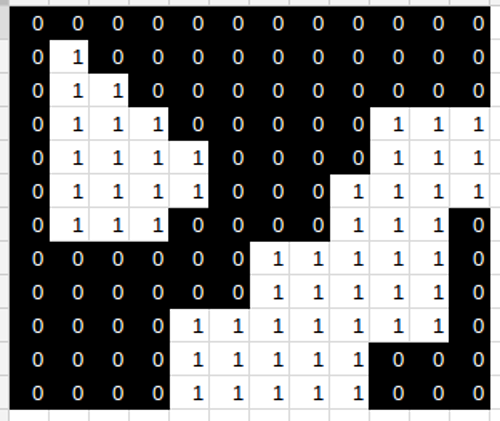
\includegraphics[scale=0.45]{pics/morphologyexample.png}
		\caption{Original Binary Image}
	\end{subfigure}
	\hfill
	\begin{subfigure}{.45\textwidth}
		\centering
		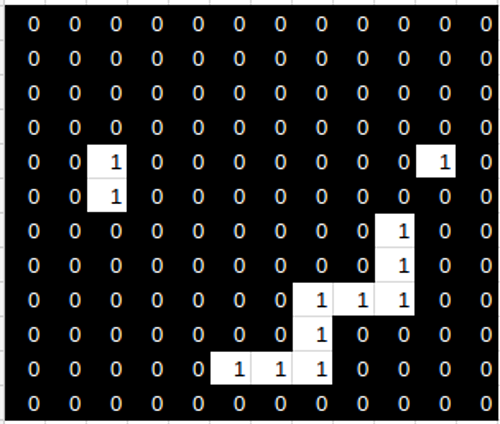
\includegraphics[scale=0.45]{pics/morphologyexample_e.png}
		\caption{Eroded Image}
	\end{subfigure}
	\label{fig:ErosionExample}
\end{figure}

\subsubsection*{Dilation}
\begin{center}
	Dilation causes bright areas of image to expand.
\end{center}
\begin{figure}
	\centering
	\begin{subfigure}{.45\textwidth}
		\centering
		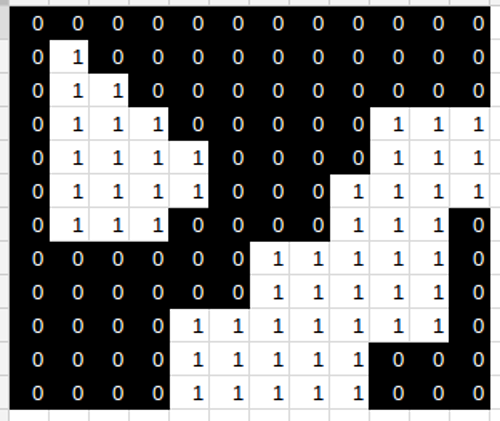
\includegraphics[scale=0.45]{pics/morphologyexample.png}
		\caption{Original Binary Image}
	\end{subfigure}
	\hfill
	\begin{subfigure}{.45\textwidth}
		\centering
		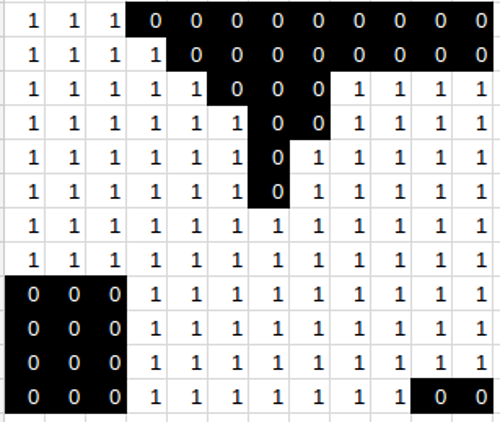
\includegraphics[scale=0.45]{pics/morphologyexample_d.png}
		\caption{Dilated Image}
	\end{subfigure}
	\label{fig:DilationExample}
\end{figure}


\subsubsection*{Closing}


\subsubsection*{Image Registration}
% Lining up the AR to the paper
\subsubsection*{Feature Abstraction}
% Possibly extracting known feature points like a house indicator







%History
%What it can do

Nowadays, technology is obsessed with being more interactive, especially in 
the realm of games and education. With the emergence of hardware such as
Google Glass and the Oculus Rift, augmented and virtual reality is becoming
a hot and exciting field in which to make technological advances. Emphasis
has been made on "immersing ourselves" within the game or environment that
we are interacting with, in order to get a much more stimulating experience
which leaves a great impression upon us. I myself had taken a liking to 
Augmented Reality (AR) sometime before applying for my M.Eng Computing degree
at Imperial College London. This original interest provided most of the 
motivation for taking up this project.

\subsection*{Investigating Hardware}
The rest of my motivation for this project came from the investigation into 
the current touchless devices and advanced displays on the market and 
available to developers and consumers alike to play around with. I looked 
into several of these hardware devices of which I now outline my findings.
 
\subsubsection*{LeapMotion}
\underline{Background \& History} \\ 
The Leap Motion company has been around since 2010, the release of their 
touchless control/ input device, the Leap Motion, was in 2013 meaning it
is a relatively new entrant into the market. However, it has generated a 
lot interest in this area of software development. The Leap Motion is one 
of the better performing touchless controls on the market and has a 
growing community of developers. The Leap Motion has an online app 
store\footnote{https://apps.leapmotion.com/} that features various games, 
apps as well as tools and utilities produced by developers and available 
for other Leap Motion owners to purchase and play with.
\\ \\
\underline{How it works} \\ 
The Leap motion comprises of 2 infrared cameras and 3 infrared LEDs,
these can be seen in figure \ref{leapmotioninteral}. After being 
placed flat on a surface, the Leap Motion emits infrared light and 
captures it back once it is reflected off surfaces, namely your hands.
The Leap Motion tracks near field infrared, making the captured images 
grayscale and able to be shown in the development kit.
The device boasts 10 finger, simultaneous tracking within a range
of around 8 cubic feet. The capture range is in a hemispherical shape
as can be observed in figure \ref{leapmotioninteractionarea}. This 
proves to be a more than suitable capture range if you are using the
device within the proximity of your computer or laptop. The Leap Motion
blog has a very good guide explaining how it operates 
\footnote{http://blog.leapmotion.com/hardware-to-software-how-does-the-leap-motion-controller-work/}.

\begin{center}
	\begin{figure}[H]
		\begin{center}
			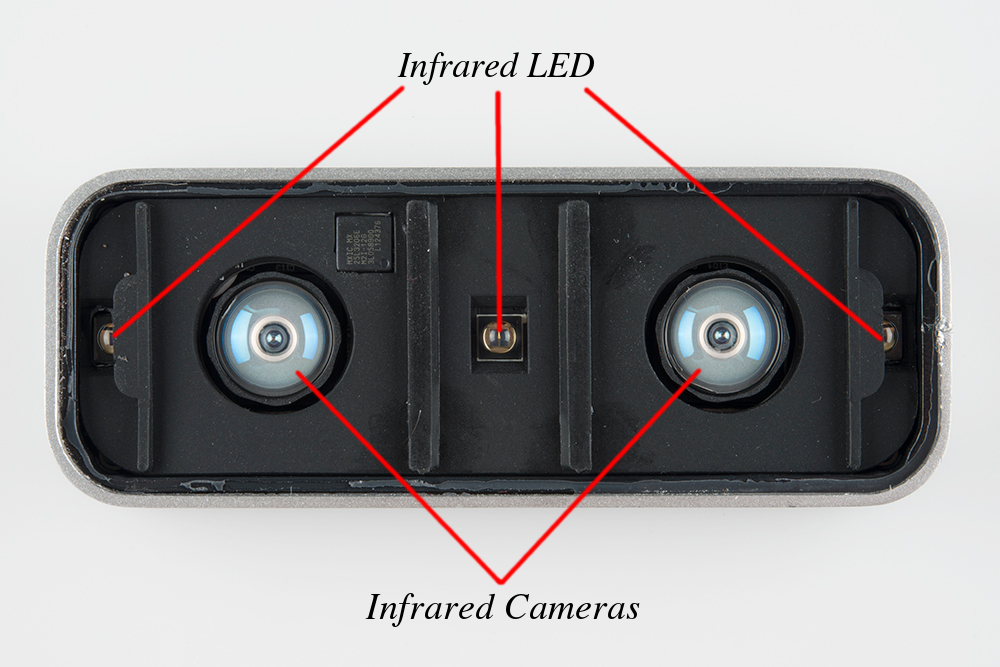
\includegraphics[scale=0.8]{pics/leapmotioninternal}
			\caption{A look inside the Leap Motion sensor}
			\label{leapmotioninteral}
		\end{center}
	\end{figure}
\end{center}

\begin{center}
	\begin{figure}[H]
		\begin{center}
			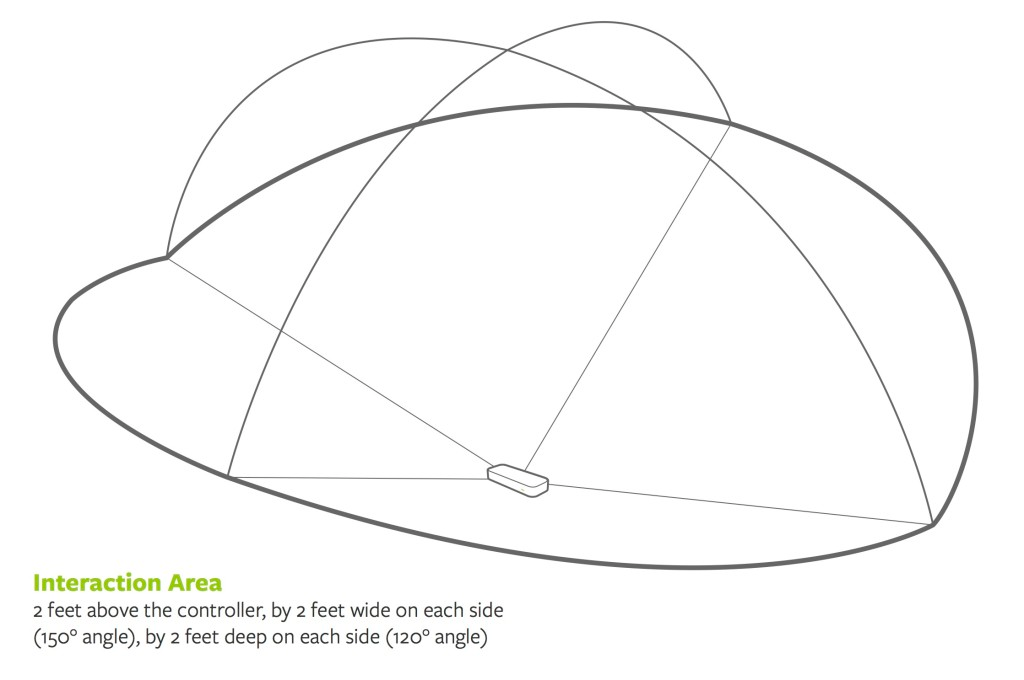
\includegraphics[scale=0.33]{pics/leapmotioninteractionarea}
			\caption{The reported range of detection of Leap Motion}
			\label{leapmotioninteractionarea}
		\end{center}
	\end{figure}
\end{center}

We can interact with the Leap Motion by placing our hands within its
capture range. If we were to move our hand past the plane on which the
infrared cameras are placed, the device registers that as a selection
by the user, equivalent to a mouse click. Any activity behind the plane,
i.e. closer to the user, will allow the user to navigate the controls.
\\ \\
\underline {My Investigations} \\
I had the chance to play around with the Leap Motion as part of my 
investigations and background research. There is a moderate community
of developers for the Leap Motion at the moment, applications are 
obtained by purchasing them on their the Leap Motion online store. 
\\ \\
There are currently 219 applications for Leap Motion as of January 
2015\footnote{https://apps.leapmotion.com/categories/all}, available
on the store. Of these, 136 are classed under \textit{Games}, 8 as 
\textit{Virtual Reality} and 42 classed as \textit{Music/Entertainment} 
(these categories are not mutually exclusive). We can take this as a 
representation of what exactly the Leap Motion is currently capable of 
doing well. Over half of the applications were aames, even more could 
technically be considered a game. 
\\ \\
The other categories of application included Education,Computer Controls,
Utilities and Creative Tools. These do not come anywhere near as close as 
the number of Game apps, Utilities was the closest with 30 apps under its
category on the store. Existing technologies and conventional methods of 
input such as webcams, mice, touch screen and keyboard are probably 
still the much faster alternative than navigating with a touchless display
for these areas of applications. Using the Leap Motion for these particular 
uses would probably be much slower and less efficient (and most of the time more 
infuriating as I have experienced first hand!) than conventional input methods.  
\\ \\
There have been a numerous amount of reviews for the Leap Motion, 
\textit{Tested}, a popular tech youtube channel, had a review concerning the
device \footnote{https://www.youtube.com/watch?v=ZK5FRPwIWVE} where they
stated the Leap Motion was "Not a mainstream device", "...just a bag
of crap; set it on fire". However, \textit{Tekzilla}, another popular Youtube 
channel which promotes new technologies offered a much better review, 
albeit, bringing in someone from the company to demo the 
device \footnote{https://www.youtube.com/watch?v=gOtAhU3DIv0}.
\\ \\
Leap Motion has also paired up with the company Oculus
\footnote{https://www.oculus.com/} to release their 2nd 
development kit. Oculus is a company specialising in the production of head
mounted devices which are used for virtual reality applications. 
The two have worked closely to allow the Leap Motion to be mounted
onto the Oculus Rift VR headpiece \footnote{https://developer.leapmotion.com/vr}.
This has opened up the possibility for a new, wide range of 
Virtual Reality Games with touchless interaction. There are already examples
of such games on the Leap Motion store. I shall not investigate further into the
Oculus as my project does not deal with virtual reality.
\\ \\
\underline{Limitations and pitfalls} \\
When using the Leap Motion, there were several things I noticed. Although the 
visuals and applications are very pretty and nice, it does not matter when the
Leap Motion decides not to work. As this company and its 
device are the best, small, double-hand motion and image capture currently out
there, there is definitely scope to manipulate what this piece of hardware offers.
\\ \\
Due to the sensors using infrared light and cameras collecting the reflected, 
emitted light, there are some very clear limitations of the Leap Motion. Infrared
light travels in straight lines, as a result, if you occlude your fingers behind
one finger, say by arranging your hand such that your thumb faces the ceiling and 
place this directly above the Leap Motion, it'll be unable to tell what your 
fingers are doing, bar the one that it can actually see. We can see evidence of
this in figure \ref{LeapMotion1} where my hand circled in red is clenched but the
Leap Motion momentarily still believes it has a finger sticking out.
\\
\begin{center}
	\begin{figure}[H]
		\begin{center}
			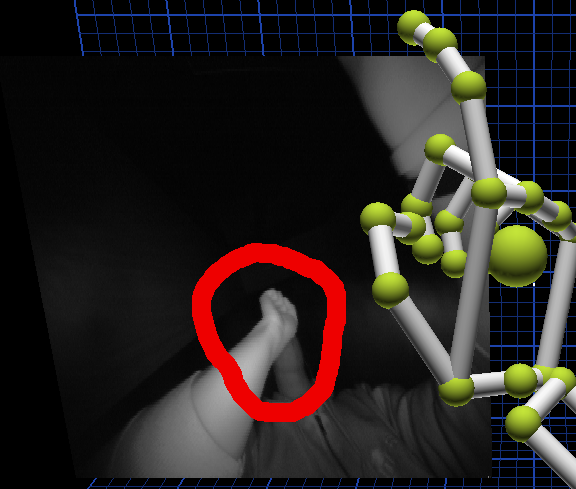
\includegraphics[scale=0.45]{pics/LeapMotion1}
			\caption{What cameras see vs skeletal hand mapping}
			\label{LeapMotion1}
		\end{center}
	\end{figure}
\end{center}

One way to try tackle this apparent problem is to use historical data, i.e.
the movement of points of the fingers over the past 3 seconds to help estimate
the position of any occluded fingers, though if this was implemented is not
at an acceptable level yet, especially if time critical, responsive 
applications require your hands to be in the positions of self occlusion. 
\\ \\
In fact,on the Leap Motion website they state that the device software will
"...interpret the 3D data and infer the positions of occluded objects. Filtering 
techniques are applied to ensure smooth temporal coherence of the data.". So infact
already do some kind of inference on the likely positions of the fingers and joints
in according to what they have managed to captured. Though it does take a few seconds,
the Leap Motion can quite accurately, under what I have managed to explore hands on with
the device, correct the input to what it actually is in real life.
\\ \\
Another noticeable limitation of the Leap Motion is its precision and ability to
deal with movements which require more finesse. Firstly, you cannot even think about
clenching or clasping your hands together as the sensor will no longer detect any hands.
In addition, it was even apparent through the demo games that the Leap Motion takes a lot
of getting used to as trying to perform small actions such as plucking a single petal,
as seen in figure \ref{leap2}, was very difficult to get right, at least in my case
and many of my friends' cases. It seems minute and delicate gesture inputs aren't captured 
and expressed very well by the Leap Motion and its current apps.

\begin{center}
	\begin{figure}[H]
		\begin{center}
			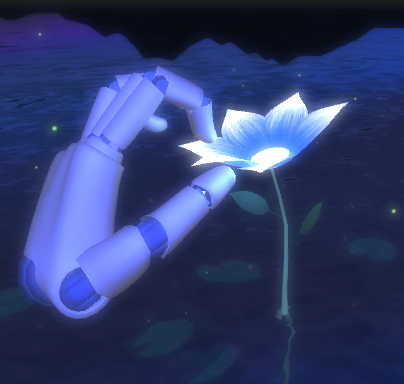
\includegraphics[scale=0.55]{pics/LeapMotion2}
				\caption{The Demo game for Leap Motion}
			\label{leap2}
		\end{center}
	\end{figure}
\end{center}

To use the device effectively, you have to place your hands in a constant 
state of being parallel to the Leap Motion such that each of your 10 fingers
can be captured by the infrared cameras. In addition, when you bring your fingers 
too close together, the sensor becomes less and less able to distinguish it 
as 2 fingers or 1, fat, finger, providing further loss of information and 
inaccurate representation of input, requiring you to be conscious of the placement
of your hands and fingers in relation the other hand or fingers.
\\ \\
Another problem arising from the infrared LED cameras is that they can absorb any
infrared light, thus in an environment where there may be external sources of 
infrared such as in the outdoors, the Leap Motion becomes less responsive and
finding it hard to properly track the fingers as the light collecting in the
camera may first be more than emitted and also will affect different parts of 
the sensor creating a grayscale image with possibly large white areas. In addition
to this problem, when indoors and your Leap Motion is pointing upwards onto a
particularly reflective ceiling or one that has an infrared light source, the same
inaccuracy happens. A very neat trick, however, is that the Leap Motion is able
to detect some discrepancies in the capture of the hands that it can suggest
to us when we might want to clean the device from finger smudges.
\\ \\
I gained further insight into the performance of the Leap Motion through the
paper \textit{Analysis of the Accuracy and Robustness of the Leap Motion 
Controller}\cite{Weichert13} which looks 
into the accuracy of the preliminary Leap Motion (release version should 
perform at least this well) and assesses its accuracy. The guys at Leap Motion 
claimed finger and movement racking to be accurate within 0.01mm. Subjecting the 
Leap Motion to average conditions, the paper concluded that although this 
claim was not likely achievable, a decent 0.7mm accuracy could still be
achieved.
\\ \\
In addition there have been a few interesting use case proposals for the
Leap Motion. One such piece is explored in the paper 
\textit{Intuitive and Adaptive Robotic Arm Manipulation using the Leap Motion Controller}
\cite{Bassily14}.
It puts forward the idea of creating a human interface with the elderly
such that they can carry out "Activities of Daily Living (ADLs)".
With the Leap Motion as input to control robotic arms, humans
actions can be mimicked by the users such that if they would otherwise not 
have the strength or coordination to perform an action, they will be able to control
the robotic arm very easily by just performing the action over the sensor. 
Those suffering from Alzheimer's or significant limb/muscle
weakness will benefit from this and the paper also talks about correcting hand
tremors and shakes from the input to provide a smooth output. 
Being only \texttt{\$80} per piece of Leap Motion device, it is 
also cheap alternative, in today's standards, to specialised sensors as well 
as its size advantage, being smaller than gyroscopes and accelerometers.  

\subsubsection*{Microsoft Kinect V2}
\underline{Background \& History}\\
The Microsoft Kinect(V1) was original released as an extra piece of hardware
for Microsoft's Xbox360 in 2010. The Kinect for windows (V2) was released
in 2012 and offered a range of improved statistics from its ancestor,
V1. Since its introduction into the market, the Kinect has received a lot of
attention from developers and there have been many applications for it put
forward\footnote{http://www.microsoft.com/en-us/kinectforwindows/meetkinect/gallery.aspx?searchv=entertainment}.
Many large companies have caught onto its capabilities and work 
alongside Microsoft and the Kinect.
\\ \\
In contrast to the Leap Motion, the Kinect V2 offers users the ability to track their 
whole body with reasonable accuracy. In addition, the V2 can track up to 6 individuals
at one time with 25 body joints able to be placed onto the captured images.
This opens up a whole new range of applications
that the Kinect can be used for and this is apparent in the amount of interest in the
Kinect, along with the amount of published papers and success stories of different
uses of it. Some of the possible fields this device can be used include 
Augmented Reality, Entertainment and Games, Retail, Education and much more. The 
Microsoft Kinect website highlights some of these interesting projects in more detail
\footnote{http://www.microsoft.com/en-us/kinectforwindows/meetkinect/default.aspx}.
\\ \\ 
The paper "Evaluation of the Spatial Resolution Accuracy of the Face 
tracking system for Kinect For Windows V1 and V2" \cite{AmonFuhrmann14}
explores in more detail the increase in performance and capability
of the V2 and shows that is beats V1 in every aspect. 
\\ \\
\underline{How it works} \\ 
The V2 allows us to take infrared images along with 1080p colour images. It 
also has depth sensors to produce depth images. Inside the V2 are 3 infrared
emitters along with a colour camera, an infrared camera and some microphones.
These internal components can be seen in figure \ref{kinectinternal}. The
microphones are along the bottom but will not be used within my project. 
\begin{center}
	\begin{figure}[H]
		\begin{center}
			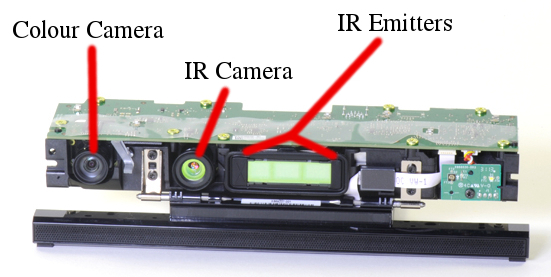
\includegraphics[scale=0.5]{pics/kinectinternal}
				\caption{Inside the Kinect V2 for Windows}
				\label{kinectinternal}
		\end{center}
	\end{figure}
\end{center}

The Kinect V2 differs from the V1 majorly in the way it produces depth maps.
V1 uses structured light while the V2 utilises Time-Of-Flight. Time-of-Flight
involves emitting many short bursts of infrared light (strobing it) and then
collecting it back through its camera. A very thorough discussion of how this
determines the depth of objects in the captured image is present on Daniel
Lau's blog \footnote{http://www.gamasutra.com/blogs/DanielLau/20131127/205820/The\_Science\_Behind\_Kinects\_or\_Kinect\_10\_versus\_20.php}.
The technique involves splitting a pixel in half and collecting infrared light
on the pixel. However, they are on at different times, while one half is on, 
the other is off and depending on the ratio of how much light is collected 
by each half (ratio since it accounts for light absorption by objects in the scene),
the relative depth of objects can be inferred. 
\\ \\
The V2 also accounts for over exposure and saturation of pixels. This scenario
occurs when there are alternative sources of infrared light, i.e. in an outdoor
environment! The V2 can reset pixel values in the middle of an exposure, also
explained in Daniel Lau's blog mentioned above. This then
allows it to be used outside where the V1 wouldn't account for this and cause
all kinds of strange behaviour; this of course means that the scope for using
the V2 and its applications is significantly larger than it ancestor.
\\ \\
\underline{My investigations} \\ \\
I investigated the Kinect for Windows first hand. In figure \ref{KinectDepth} 
you can see an example of the depth sensing capability of V2. On the right,
circled in blue, is myself. I sat around 40cm away from the camera. As I highlight 
in the limitations section below, this is reported as the minimum distance 
performance can be guaranteed by the V2. My friend, Juto Yu, is circled in 
yellow, he say slightly outside the view of the camera, giving me a rough 
indication on how wide the capture region is. The green circled object is a 
pillar in the central library of Imperial College, it is definitely more than 
3m away from the V2 which is reported as the range before objects become 
"too far". Whether it being detected is because the device can actually 
handle larger caption depths or due to the pillar being white and thus 
more reflective will need to be further looked in to.
\begin{center}
	\begin{figure}[H]
		\begin{center}
			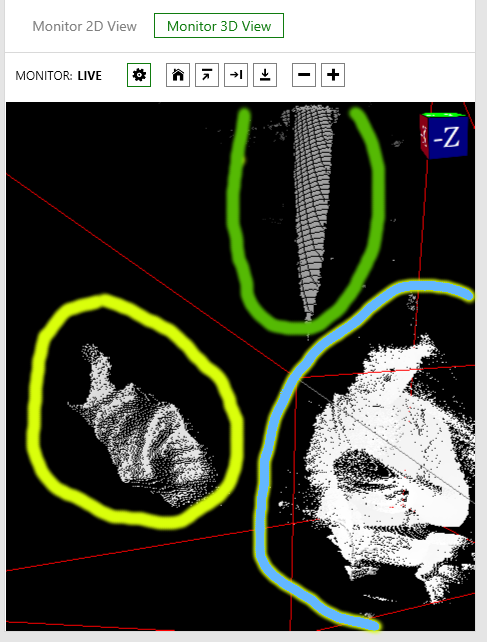
\includegraphics[scale=0.5]{pics/KinectDepth}
				\caption{Depth image from Kinect V2}
				\label{KinectDepth}
		\end{center}
	\end{figure}
\end{center}

I also looked into the colour camera's performance. The camera has a 1080p HD
video taking capability and is of a good quality. In addition, as seen in 
figure \ref{KinectColour}. The body tracking is pretty good and can make rather
accurate implications of people's limbs even when they are sitting down and are
obscured as shown. I was sitting at a desk but the V2 could make some guesses
as to where my legs would be. It is also clear that multiple tracking can be done
in real time at a speed that is responsive.
\begin{center}
	\begin{figure}[H]
		\begin{center}
			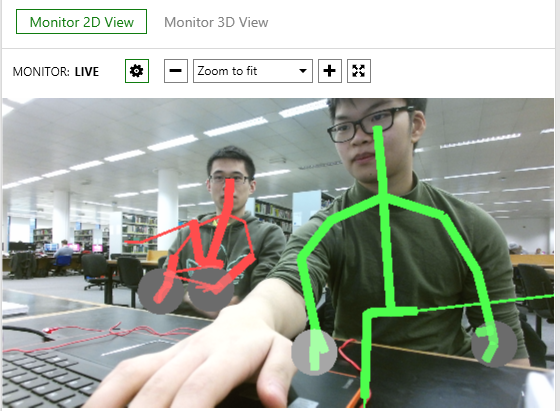
\includegraphics[scale=0.5]{pics/KinectColor}
				\caption{Colour Camera (with body tracking)}
				\label{KinectColour}
		\end{center}
	\end{figure}
\end{center}

The V2 is definitely a great alternative to some of the more expensive depth 
sensors on the market. As highlighted in the paper
"Low-cost commodity depth sensor comparison and accuracy analysis" by
Timo Breuer, Christoph Bodensteiner, Michael Arens. Some of the other sensors
that out perform it are upwards of £3000 while the V2 costs just around £150.
This means that it will be accessible to a much larger audience, something
definitely needed if an Augmented Reality game is to be successful.
\\ \\
\underline{Limitations and pitfalls}\\
The cameras of the V2 have a set range of values that it works well within.
This is reported by Microsoft to be from 0.4m to 3m
\footnote{https://msdn.microsoft.com/en-us/library/hh973078.aspx\#Depth\_Ranges}.
Anywhere beyond that seems to be too
far to determine the depth of objects. There is also a notion of being too near
to the device to! If we are working with the device, say, next to our laptop or
in a space nearby, there may be complications with how the sensor performs, 
anything closer than 0.4m produces unknown behaviour with the depth sensor.
\\ \\
A pitfall I expect to encounter is when developing with the Kinect SDK. I have
experience in C++ which is one of the languages that can be used to write Kinect 
applications. However, it seems a lot of the colour camera tutorials are written
in C\# which will could cause problems for me if I had to pick up the language 
or translate it into the C++ equivalents. However, this should only be a small
pitfall and cause minor hindrance to the progression of the project.

\newpage

\subsection*{Anticipated End State}
With this hard deadline in mind, I need to set a state of the project which I think
I would have reached by the deadline. Past this I do not aim to make any significant
changes bar running tests for evaluations, which means that my code has to be 
pretty much bug proof by this date.
\\ \\
Of course I would have hoped to finished all of the objectives I set out in the 
beginning of this report. However, if things do not progress as quickly as you
would like them on any project. I will put more focus into the Augmented Reality
part of the project. Integrating the Leap Motion and the touchless manipulation
of the created landscape is not necessary for the project to offer a novel gaming
experience. The game can lie within the creation of the landscape from a user
drawn 2D landscape and have that come to life by using the Kinect. 
\\ \\
I would definitely like to reach the point in the project where a someone can
create a 3D AR landscape. I expect the bulk of the work will lie within this 
part of the project as there is a lot to do with image processing to complete
this step. The creation of the landscape may also take some time as I am still
unfamiliar with what I should use to create this for the user. 
The next major milestone will be extending this point to provide the created 
landscape with an illumination model that is equivalent to the scene it is being
portrayed within. I expect this also to take up a fair time, however, since
I am learning about it within a module of my course right now, hopefully I 
will be able to grasp its concepts faster than without. Making amendments to the
illumination should take a bit of time. Past this point I shall consider as 
extensions to the project that would be great to implement. Though the 
investigation and project will concentrate on the two points above.

\subsection*{Extensions}
I have two planned extensions for this project immediately on completion. 
The first of which is that after the render of the first Augmented
Reality scene, the user can choose to fix that in place (though rotation and
translation of the scene can still take place) and then introduce 
modifications to the scene in real life. For example, placing in a pencil case,
a water bottle or even a scrunched up piece of paper. This will then reflect 
upon the AR scene. Imagine it as you being a Giant, playing around with the
AR world that you have created. The scene should change with the introduction
of this new object, this will include occlusions, different shading and light to
name the main challenges.

The next extension would be to allow you to interact with the landscape using
the touchless input device, Leap Motion. What exactly this will entail has not
yet been set in stone but some ideas I have are the following:
\begin{itemize}
	\item Allowing the user to add accessories or other landforms onto the
		  scene by selection and direct placement. Imagine it as the Sims or
		  any other simulation game where you can choose to build a house, etc.
		  on the scene.
	\item Introducing randomly generated content such as miniature people, 
		  avatars, objects etc. to traverse the landscape which can then be
		  manipulated and moved around. 
	\item Allowing the user to use view their hands in the scene, kind of like
		  they were playing God, allowing them to interact with the scene, for
		  example if they spread their hands, it could cause rain on the scene.
\end{itemize}

One other extension which is pretty ambitious would be to track the original 
feature drawing you provide to generate the first AR image. After that, if the
user deforms this image, the scene will deform alongside. This means that
extending past drawing on more features, if the user scrunches up the paper,
tears it in half or transforms it in some way, allow the scene to change such 
that it reflects the difference in between the before and after of the feature
drawing. For example, tearing the drawing will cause a rip to form in the 
generated landscape. Deforming the drawing will deform the landscape. In
essence, this will be taking feature points of a feature drawing!
\newpage
\section*{Evaluation Plan}
The below shall outline my evaluation plan of this project. It is important my 
evaluation is rigorous and solid so that it proves that what I would've produced at
the end is something others can use and build upon. This is because if I am to 
provide any kind of advances in this field, then what I produce must be proven to 
be sound. I will be basing my Evaluation plan over the points I outlined in my
anticipated end state in my project plan.

\subsection*{Indicators of Success/Benchmarks}
\subsubsection*{Functionality}
At the end of this project, I hope that I am able to quickly draw
up a feature drawing on a piece of paper within 3 minutes (5 minutes if they
want to be interesting and have a nice landscape!). I should then be able to 
place this in front of the Kinect device and have my created piece of 
software read the image and produce Augmented Reality landscape within some
acceptable time, for example within 1 minute the Landscape should have been
created and displayed. This is important because for AR to be effective and
even useful in any real life application, it has to be fast and responsive,
being close to real time as possible. In addition, since the main motivator
of this project is that current AR applications do not look realistic enough.
I hope that by the end of this project I can produce a landscape that looks
realistic, at least in terms of illumination.

\subsubsection*{User Testing}
For any game to be considered anywhere near success, user testing needs to 
take place. I intend to test the software on a range of people, from those not
technically inclined to the younger generation, including children! Hopefully
I can then ascertain the age groups to which this can be marketed to. If the
feature drawings require a relatively high amount of detail, then young children
are likely to find troubles with getting what they want out of the software.
Hopefully through user testing I can also discover faults, possible extensions,
improvements and edge cases. I'd like to set the number of test subjects as at
least 20 individuals, of which multiple testing will occur.

\subsubsection*{Responsiveness}
To further enforce what I mentioned in Functionality, there will be a whole 
other set of evaluation criteria I set out to assess the success of my project.
The first of which is responsiveness of software, which is what I mentioned 
above. The software should generate the illuminated 3D landscape within a 
minute of being presented the feature drawing. An even better turnover would
be ideal, hopefully within the range of 15 seconds as even a minute is long to
wait for an Augmented Reality game.

The software should also be able to detect rotation of the feature drawing
and also rotate the landscape as appropriate. This would ideally be a lot more
responsive than the target above, within the 2 second range. Any more and the
movement would look choppy and will not represent an accurate rotation. However,
as the illumination model is a lot more advanced, this may or may not be 
possible, considering some very basic Augmented Reality applications don't even
react this fast in the presence of rotation. This rotation should also reflect in 
the shadows of the landscape.

\subsection*{Testing}
\subsubsection*{Functionality}
To give qualitative and quantitative results to the evaluation criteria I have 
proposed above, first it is very easy to just measure the time it takes for the
software to generate the 3D landscape and then see how long it takes from
the moment the user presents their feature drawing to the Kinect. How close the
performance is to the time boundaries I have outlined above will determine how
well the software and project can be deemed a success. However, the rate of
success will have an exponential relation to deviance from the set boundary.
This is because if it gets too slow, it would cause much anger and frustration 
to the users of the software because as I have mentioned already within this 
report, AR and its growth and success heavily depends on being next to real time.
To give an idea, if I rotated the scene, then if it took above 5 seconds to reflect
the change in the landscape, this is way too slow to be of any use or of any fun.
This will be a failure.

\subsubsection*{User Testing}
Being a game and very much a visual project, feedback will be needed from a 
numerous amount of people due to the subjectiveness of these criteria. 
Written feedback in the style of questionnaires would be a good way to
quantify the performance of my project by the people I will be asking to take
part in my tests. 

\subsubsection*{Responsiveness}
The responsiveness can be tested against some hard time boundaries, once again
with their exponential penalty the more time it is from the the boundary. This
can easily be tested by tracking how much time it takes between tested actions.
When it comes to the assessing the responsiveness of the illumination change,
this can be measured by eye, if the illumination stays consistent with the 
lighting in the scene, then generally this can be considered a success. If the
scene looks realistic and the shadow placement makes sense and obscured 
areas become visible on rotation, then these are also indicators that it passes
the test. The realism of a scene is a lot more subjective and therefore, as 
mentioned above, the test will range over a set amount of people. If the majority
thinks the scene still looks real after a change, we can consider this a success.


\bibliographystyle{plain}
\bibliography{biblio}
\end{document}
